\chapter{Implementação}
\label{chap:implementacao}
Para comparar os sistemas que utilizam apenas um banco de dados (persistência monoglota) com os sistemas que utilizam mais de um banco de dados (persistência poliglota) implementamos e testamos o desempenho desses. Escolhemos fazer uma aplicação semelhante ao Twitter. Nessa aplicação, o usuário poderá se cadastrar, escrever \textit{tweets}, seguir outros usuários e listar os \textit{tweets} dos usuários que ele segue. Este capítulo é dividido em duas seções, a primeira, \autoref{sec:useCase} descreve os casos de uso da aplicação. A \autoref{sec:applications} descreve os detalhes da implementação com persistência monoglota e com persistência poliglota.

\section{Casos de Uso}
\label{sec:useCase}
Essa seção irá descrever os casos de uso da aplicação. Cinco subseções foram criadas para detalhar os cinco casos de uso criados. A primeira \autoref{subsec:useCaseCreateUser}, detalha o caso de uso que descreve a funcionalidade de cadastro do usuário. A \autoref{subsec:useCaseCreateTweet} descreve o caso de uso de cadastro de um \textit{tweet}. A \autoref{subsec:useCaseUserFollow} apresenta o caso de uso que descreve como o usuário segue outro usuário. A \autoref{subsec:useCaseUserUnfollow} apresenta o caso de uso que descreve como o usuário para de seguir outro e por fim, a \autoref{subsec:useCaseFeed} descreve o último caso de uso que detalha como o usuário visualiza o \textit{feed}, página que apresenta todos os \textit{tweets} dos usuários que o usuário logado segue.


\subsection{Caso de Uso 1 - Cadastro do usuário}
\label{subsec:useCaseCreateUser}

Sumário: Usuário usa o sistema para se cadastrar

Ator primário: Usuário

Ator secundário: Sistema

Precondições: O usuário deverá ter uma conta de email


Fluxo Principal\begin{enumerate}
{\setlength\itemindent{25pt}
    \item O usuário acessa o sistema;
    \item O sistema exibe a tela de entrada, como mostrado na \autoref{fig:telaInicial};
    \item O usuário clica em \textit{Sign up};
    \item O sistema retorna a tela com o formulário de cadastro de usuário, como mostrado na \autoref{fig:signup};
    \item O usuário preenche os campos de nome, email, senha e confirmação de senha;
    \item O sistema cria o usuário e redireciona para tela de \textit{My Tweets}, como mostrado na \autoref{fig:myTweets}.
}
\end{enumerate}

Fluxo de Exceção (5): Email inválido
\begin{enumerate}
{\setlength\itemindent{25pt}
\item Se o usuário não digitou um email válido, o sistema reporta o campo incorreto e retorna ao passo 5.
}
\end{enumerate}

Fluxo de Exceção (5): Campos obrigatórios não preenchidos
\begin{enumerate}
{\setlength\itemindent{25pt}
\item Se o usuário não preencher todos os campos, o sistema informa que os campos são obrigatórios e o usuário retorna ao passo 5.
}
\end{enumerate}

Fluxo de Exceção (5): Senha e confirmação de senha não conferem
\begin{enumerate}
{\setlength\itemindent{25pt}
\item Se o usuário não preencher as senhas corretamente, o sistema retorna ao passo 5, informando que as senhas não conferem.
}
\end{enumerate}

\begin{figure}[H]
    \centering
    \caption{Tela Inicial}
    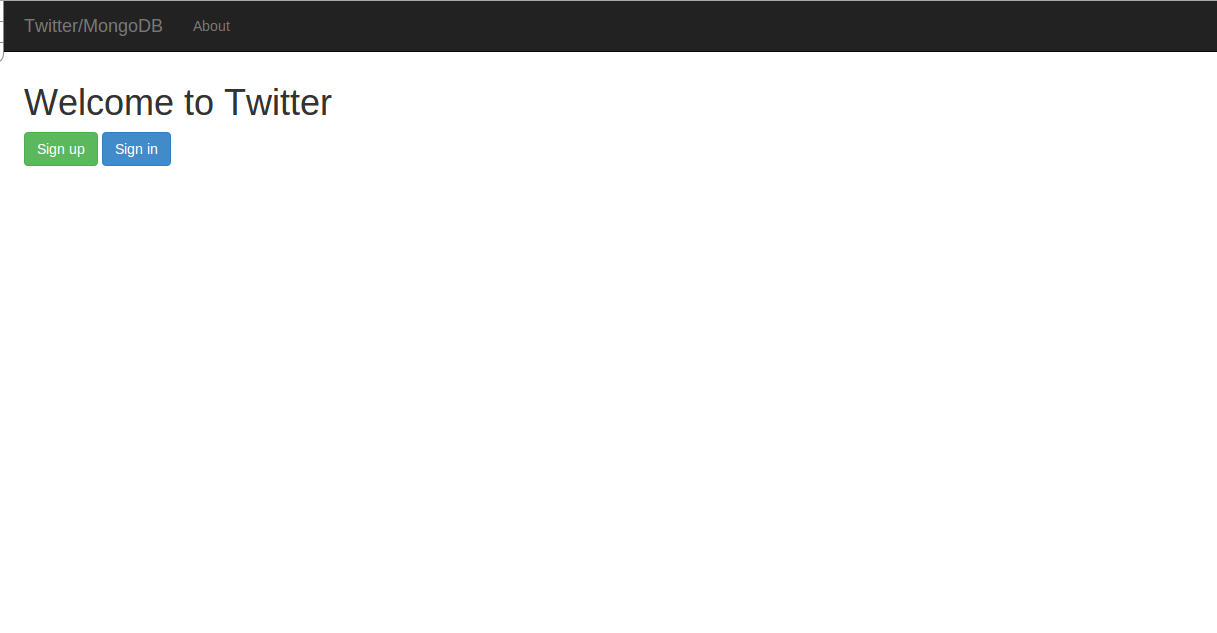
\includegraphics[width=0.8\textwidth]{./04-figuras/PrimeiraTela.png}
    \label{fig:telaInicial}
\end{figure}

\begin{figure}[H]
    \centering
    \caption{Tela de cadastro de usuário}
    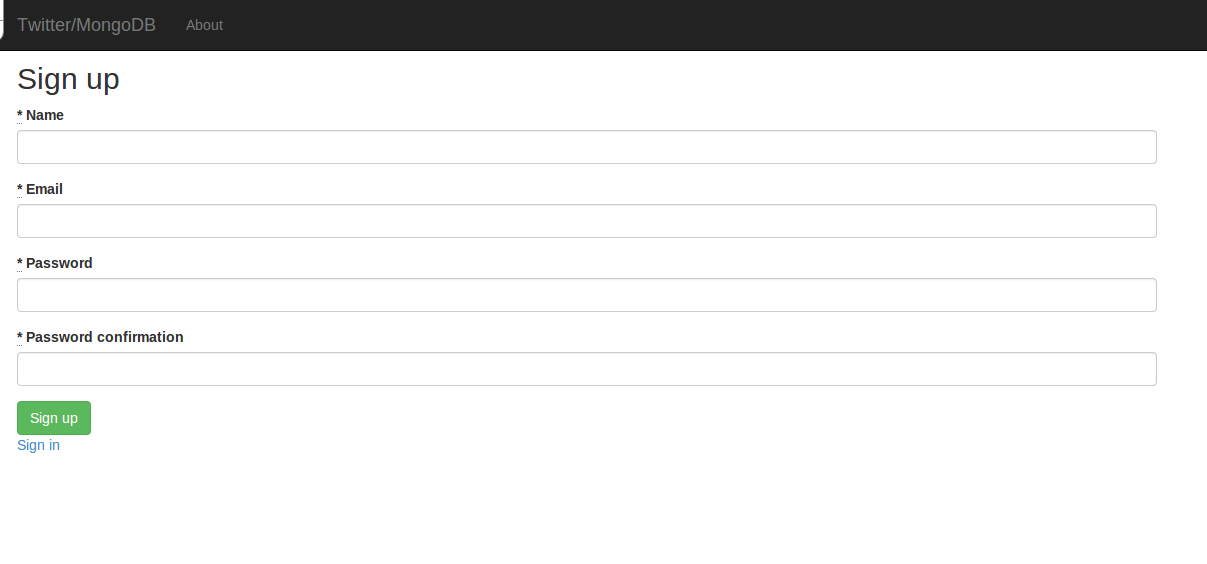
\includegraphics[width=0.8\textwidth]{./04-figuras/Signup.png}
    \label{fig:signup}
\end{figure}

\begin{figure}[H]
    \centering
    \caption{Tela Tweets do Usuário Logado}
    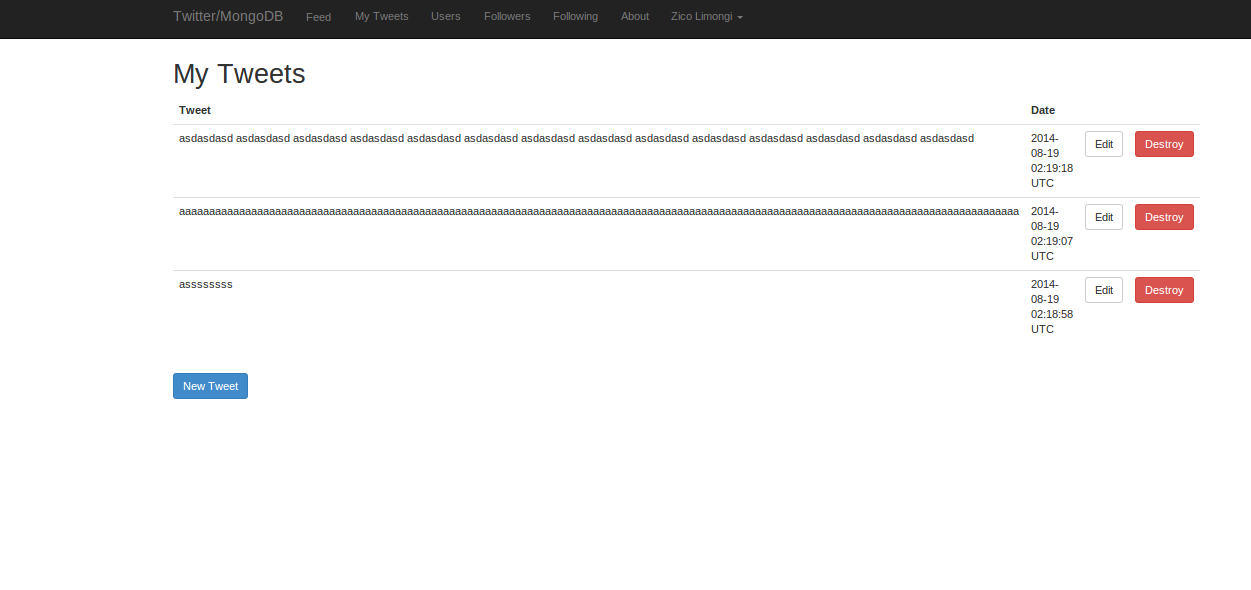
\includegraphics[width=0.8\textwidth]{./04-figuras/myTweets.png}
    \label{fig:myTweets}
\end{figure}

\subsection{Caso de Uso 2 - Cadastro de \textit{tweet}}
\label{subsec:useCaseCreateTweet}

Sumário: Usuário usa o sistema para cadastrar um \textit{tweet}

Ator primário: Usuário

Ator secundário: Sistema

Precondições: O usuário deverá ser cadastrado e deve estar logado no sistema

Fluxo Principal
\begin{enumerate}
{\setlength\itemindent{25pt}
\item O usuário acessa o sistema e faz o \textit{login}, como mostrado na \autoref{fig:login};
\item O sistema abre a listagem dos \textit{tweets} do usuário, como mostrado na \autoref{fig:myTweets};
\item O usuário clica no botão \textit{New Tweet};
\item O sistema retorna com o formulário para cadastrar \textit{tweet}, como mostrado na \autoref{fig:createTweet};
\item O usuário escreve o \textit{tweet} no campo indicado;
\item O sistema cria um novo \textit{tweet}, registrando que o usuário é o autor do \textit{tweet}, data e hora que foi criado.
}
\end{enumerate}
\begin{figure}[H]
    \centering
    \caption{Tela de Login}
    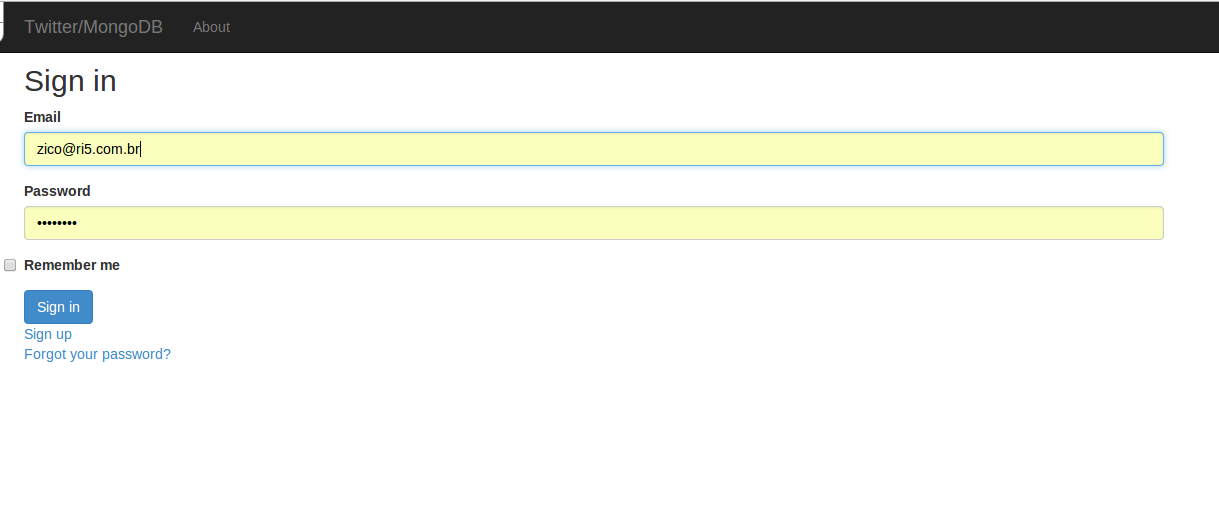
\includegraphics[width=0.8\textwidth]{./04-figuras/login.png}
    \label{fig:login}
\end{figure}
\begin{figure}[H]
    \centering
    \caption{Tela Cadastro de Tweet}
    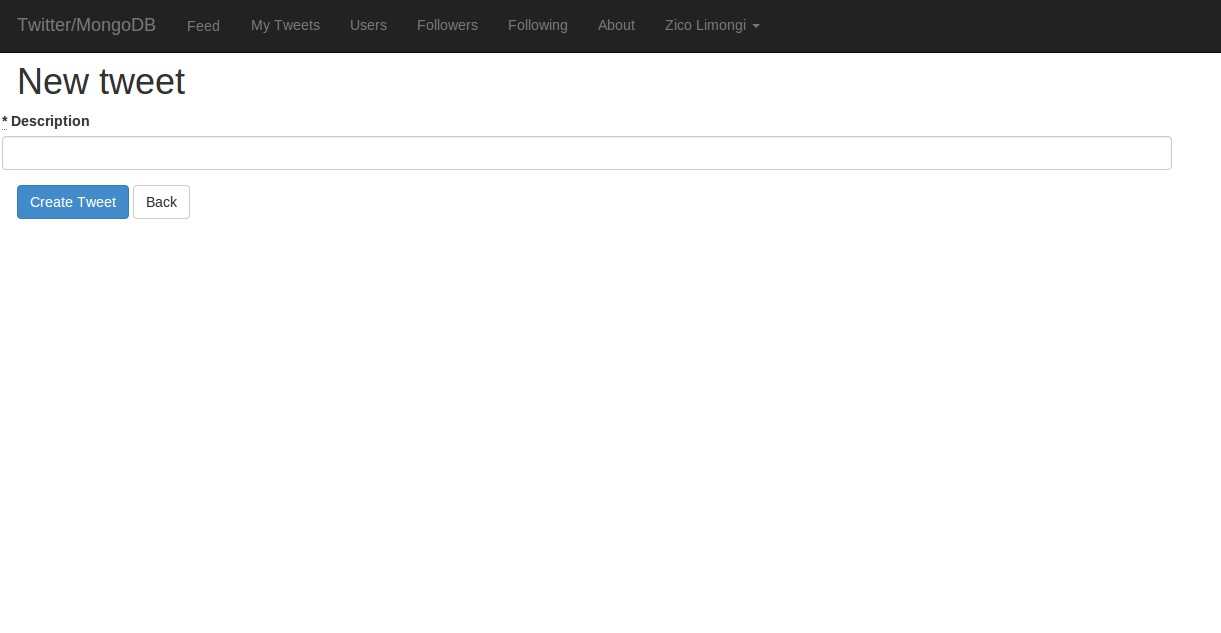
\includegraphics[width=0.8\textwidth]{./04-figuras/createTweet.png}
    \label{fig:createTweet}
\end{figure}


\subsection{Caso de Uso 3 - Usuário segue outro usuário}
\label{subsec:useCaseUserFollow}

Sumário: Usuário segue outro usuário

Ator primário: Usuário

Ator secundário: Sistema

Precondições: O usuário deverá ser cadastrado e deve estar logado no sistema

Fluxo Principal
\begin{enumerate}
{\setlength\itemindent{25pt}
\item O usuário acessa o sistema e faz o \textit{login}, como mostrado na \autoref{fig:login};
\item O sistema abre a listagem dos \textit{tweets} do usuário, como mostrado na \autoref{fig:myTweets};
\item O usuário clica no menu \textit{Users};
\item O sistema retorna a listagem paginada com todos os usuários cadastrados, como mostrado na \autoref{fig:users};
\item O usuário escolhe algum usuário que deseja seguir e clica no botão \textit{Follow};
\item O sistema armazena essa informação.
}
\end{enumerate}

\begin{figure}[H]
    \centering
    \caption{Tela de Listagem de Usuários}
    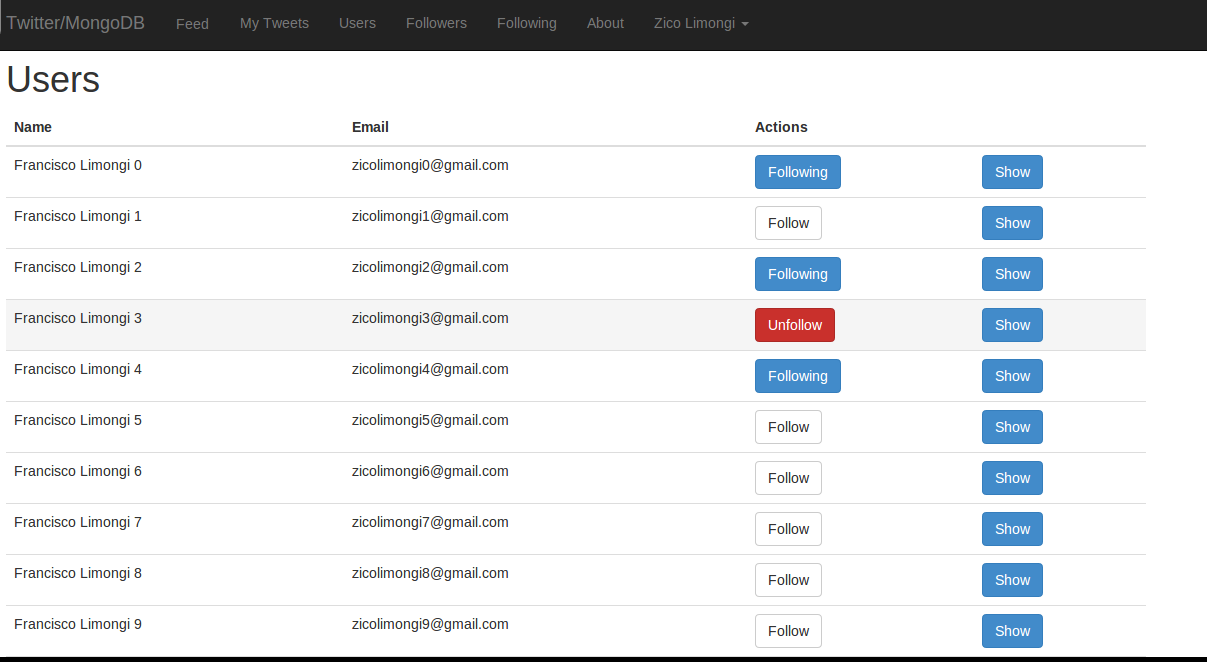
\includegraphics[width=0.8\textwidth]{./04-figuras/users.png}
    \label{fig:users}
\end{figure}

\subsection{Caso de Uso 4 - Usuário pára de seguir algum usuário}
\label{subsec:useCaseUserUnfollow}

Sumário: Usuário pára de seguir algum usuário

Ator primário: Usuário

Ator secundário: Sistema

Precondições: O usuário deverá ser cadastrado e deve estar logado no sistema. Além disso, o usuário logado deve estar seguindo o usuário que ele deseja parar de seguir

Fluxo Principal
\begin{enumerate}
{\setlength\itemindent{25pt}
\item O usuário acessa o sistema e faz o \textit{login}, como mostrado na \autoref{fig:login};
\item O sistema abre a listagem dos \textit{tweets} do usuário, como mostrado na \autoref{fig:myTweets};
\item O usuário clica no menu \textit{Users};
\item O sistema retorna a listagem paginada com todos os usuários cadastrados, como mostrado na \autoref{fig:users};
\item O usuário encontra o usuário que deseja parar seguir e clica no botão \textit{Unfollow};
\item O sistema armazena essa informação.
}
\end{enumerate}

\subsection{Caso de Uso 5 - Usuário visualiza o \textit{feed}}
\label{subsec:useCaseFeed}

Sumário: Usuário visualiza os \textit{tweets} dos usuários que ele segue

Ator primário: Usuário

Ator secundário: Sistema

Precondições: O usuário deverá ser cadastrado e deve estar logado no sistema. Além disso, o usuário logado deve estar seguindo algum usuário

Fluxo Principal
\begin{enumerate}
{\setlength\itemindent{25pt}
\item O usuário acessa o sistema e faz o \textit{login}, como mostrado na \autoref{fig:login};
\item O sistema abre a listagem dos \textit{tweets} do usuário, como mostrado na \autoref{fig:myTweets};
\item O usuário clica no menu \textit{Feed};
\item O sistema retorna a listagem paginada com todos os \textit{tweets} dos usuários que o ator primário segue, como mostrado na \autoref{fig:feed}.
}
\end{enumerate}

\begin{figure}[H]
    \centering
    \caption{Tela de Feed}
    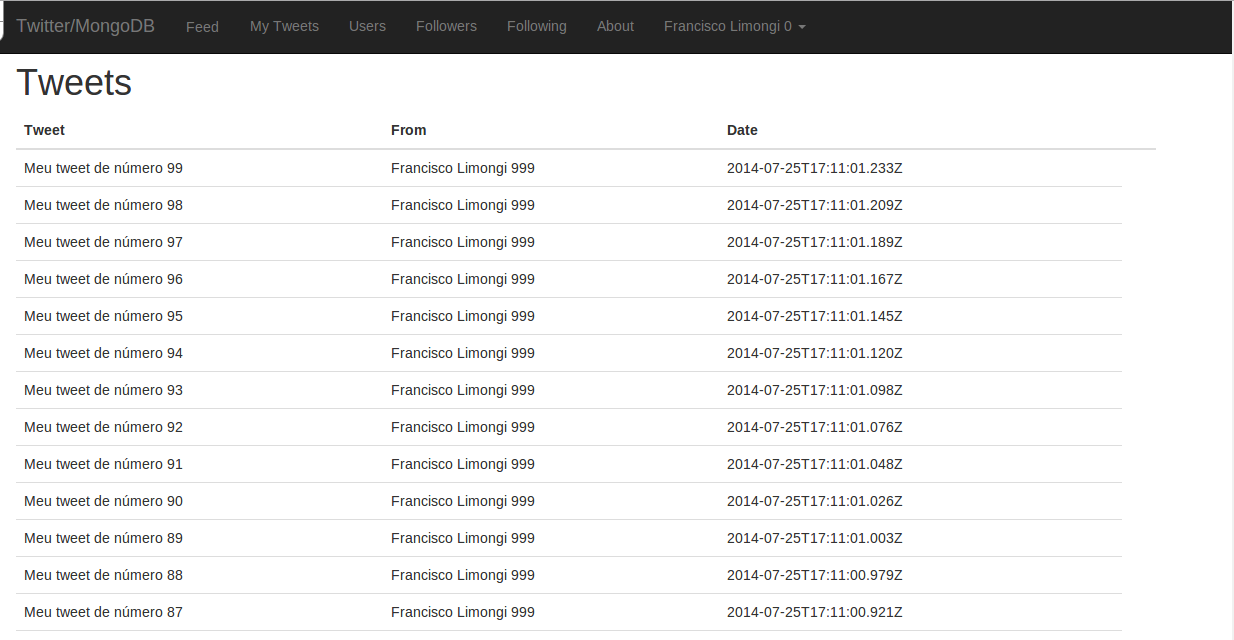
\includegraphics[width=0.8\textwidth]{./04-figuras/feed.png}
    \label{fig:feed}
\end{figure}


\section{Sistema Desenvolvido}
\label{sec:applications}

Ambos os sistemas foram desenvolvidos na linguagem \textit{Ruby} com o \textit{framework Rails}. Esse \textit{framework} é próprio para Web e utiliza a arquitetura de \textit{software} \ac{MVC}. Além disso, é uma ferramenta de desenvolvimento ágil, que facilita o desenvolvimento Web.
Foram utilizado outras \textit{gems}\footnote{\textit{Gem} é um pacote de \textit{software} que contém uma aplicação em \textit{Ruby} ou uma biblioteca. \url{http://guides.rubygems.org/}}, a lista utilizada em cada aplicação criada se encontra no arquivo chamado Gemfile.lock. Podemos destacar a \textit{gem} Devise\footnote{\url{https://github.com/plataformatec/devise}} e a \textit{gem} MongoId\footnote{\url{http://mongoid.org/}} como principais. A \textit{gem} Devise faz o controle de sessão do usuário e a Mongoid abstrai para o desenvolvedor a comunicação com o banco de dados MongoDB. Também utilizamos a \textit{gem} bootstrap-sass para melhorar a usabilidade da aplicação.

Esta seção foi dividida em duas subseções. A \autoref{subsec:monoglot} descreve os detalhes de implementação do sistema monoglota. e a \autoref{subsec:polyglot}  descreve os detalhes da implementação poliglota. A seguir apresentamos os detalhes de implementação de cada sistema.

\subsection{Implementação com Persistência Monoglota}
\label{subsec:monoglot}

Essa implementação utiliza apenas o banco de dados MongoDB que é orientado a documento. O código da aplicação está disponível no GitHub\footnote{\url{https://github.com/zicolimongi/Twitter-Mongo}}.

Na camada de modelos temos apenas duas classes, \verb|Tweet| e \verb|User|. A classe \verb|Tweet| representa o \textit{tweet} e a classe \verb|User| representa o usuário. Ambos são armazenados como coleção no MongoDB. Cada objeto de uma dessas classes é um documento. Na \autoref{fig:diagrama_models} podemos visualizar o relacionamento entre as classes.
\begin{figure}[H]
    \centering
    \caption{Camada de modelo}
    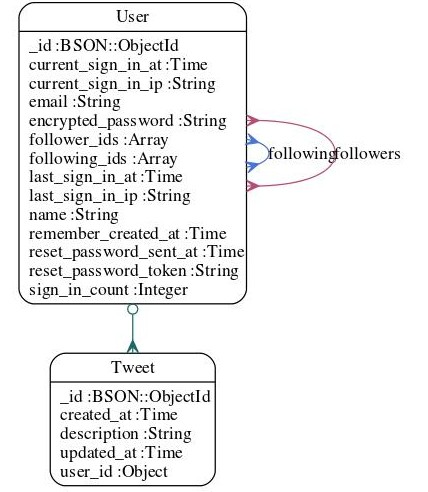
\includegraphics[width=0.5\textwidth]{./04-figuras/models_complete.jpg}
    \fonte{\cite{NoSQL}}
    \label{fig:diagrama_models}
\end{figure}
A classe \verb|Tweet| armazena o identificador do próprio \textit{tweet}, data de criação, data da última atualização desse objeto, descrição do \textit{tweet} e o identificador do usuário que criou o \textit{tweet}. Não escolhemos usar agregação nessa relação, pois umas das principais perspectivas é visualizar os \verb|Tweets| de diferentes usuários. Nessa classe, temos duas validações: uma de presença do campo descrição e outra que limita o tamanho desse campo em cento e quarenta caracteres.

A classe \verb|User| armazena o identificador do usuário, email, nome, uma série de campos usados para autenticação, data de criação do objeto, data da última modificação do objeto, lista de usuários seguidos e a lista de usuários que seguem. A classe \verb|User| tem três relacionamentos: um com \verb|Tweet| que já foi citado e dois autorrelacionamentos para armazenar a lista de usuários que seguem e que são seguidos. Esse autorrelacionamento no banco de dados orientado a documento funciona de uma maneira diferente do banco de dados relacional.
Enquanto no modelo relacional é necessário criar uma nova tabela, no modelo não-relacional armazenamos apenas as listas com os identificadores dos usuários, pois é permitido atributos multivalorados. Logo, basta armazenar os identificadores da relação em uma lista embutida no documento do usuário. Então temos uma lista que armazena os identificadores dos usuários que são seguidos, chamada de \verb|following| e outra lista com os identificadores dos usuários que são seguidores, chamada de \verb|followers|.
Essa classe tem três validações de presença: uma para o campo nome, outra para o campo email e a terceira para o campo de senha.

Na camada de controle temos uma hierarquia de classes conforme mostra a \autoref{fig:diagrama_controllers}. \verb|ApplicationController| é a classe de controle que herda da classe do \textit{framework}. Em seguida, temos o \verb|HomeController| e \verb|Logged::BaseController| que herda  da classe \verb|ApplicationController|. \verb|HomeController| é a classe responsável por implementar o controle das páginas de \verb|about| e \verb|index|. Já o controle \verb|Logged::BaseController| é a classe responsável por carregar o layout do usuário logado e verificar a autenticidade do usuário.
Abaixo do \verb|Logged:BaseController| foram criadas mais duas classes: \verb|TweetsController| e \verb|UsersController| que implementam os controles de \textit{tweets} e usuários respectivamente.
\begin{figure}[H]
    \centering
    \caption{Camada de controle}
    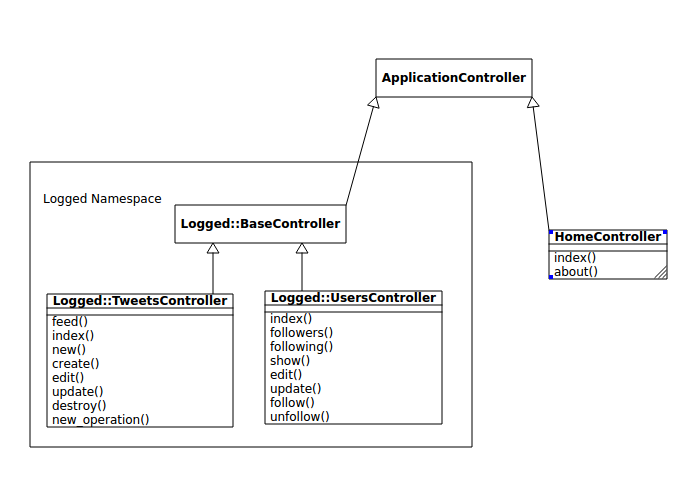
\includegraphics[width=0.8\textwidth]{./04-figuras/controllers_complete.png}
    \fonte{\cite{NoSQL}}
    \label{fig:diagrama_controllers}
\end{figure}

Toda consulta que resulte em mais de trinta registros é paginada, isto é, colocamos um limite para que o banco não busque mais que 30 registros de uma só vez. Isso funciona manipulando duas variáveis \verb|offset| e \verb|limit|. Também devemos ressaltar que
antes de todas ações é executada uma consulta, no banco, que carrega para a variável \verb|current_user| o usuário logado, caso exista. Essa busca é feita pela \textit{gem} Devise e é transparente para o desenvolvedor.

O controle de usuário implementa as ações \verb|index|, \verb|followers|, \verb|following|, \verb|show|, \verb|edit|, \verb|update|, \verb|follow| e \verb|unfollow|, todas descritas a seguir:

A ação \verb|index| lista todos os usuários com exceção do usuário logado. Na página renderizada, o usuário logado poderá seguir os usuários que ele ainda não segue, ou poderá parar de seguir os usuários que ele segue. É realizada uma consulta para ler os usuários do sistema.

A ação \verb|followers| lista todos os usuários que seguem o usuário logado. Na página renderizada, o usuário logado poderá seguir os usuários que ele ainda não segue, ou poderá parar de seguir os usuários que ele já segue. É realizada uma consulta no banco de dados que busca todos os usuários que o usuário logado segue.

A ação \verb|followings| lista todos os usuários que o usuário logado segue. Na página renderizada, o usuário logado poderá parar de seguir os usuários que ele segue. Nessa ação é realizada uma consulta, porém se busca os usuários que seguem o usuário logado.

A ação \verb|show| recebe um identificador como parâmetro e localiza o usuário que possui esse identificador. A página renderizada mostra o nome e email do usuário localizado e os \textit{tweets} que ele fez. Nessa página, são realizadas duas consultas, uma que busca o usuário e outra que busca os \textit{tweets} desse usuário.

A ação \verb|edit| renderiza o formulário de edição para que o usuário logado possa mudar algum campo, como nome, email ou senha. Nessa ação nenhuma consulta adicional é feita.

A ação \verb|update| recebe os parâmetros das alterações que o usuário fez no próprio perfil e registra isso no banco de dados. É realizada uma escrita no banco de dados para atualizar esses dados passados por parâmetro.

A ação \verb|follow| recebe como parâmetro o usuário que será seguido pelo usuário logado e registra esse relacionamento. Para isso é necessário uma consulta para ler qual usuário será seguido e duas escritas: uma para atualizar o usuário que está sendo seguido com o identificador do usuário seguidor e outra para atualizar o usuário seguidor com o identificador do usuário seguido.

A ação \verb|unfollow| recebe como parâmetro o usuário que deixará de ser seguido pelo usuário logado e apaga o registro desse relacionamento. Para isso é necessário uma consulta para ler o usuário que deixará de ser seguido e duas escritas no banco de dados: uma para atualizar a lista de seguidores do usuário que deixou de ser seguido outra para atualizar a lista de seguindo do usuário seguidor que deixou de seguir.

O controle de \textit{tweets} implementa as ações \verb|feed|, \verb|index|, \verb|new|, \verb|edit|, \verb|update| e \verb|destroy|, descritas a seguir:

A ação \verb|feed| é responsável por fazer a busca no banco de dados dos \textit{tweets} de todos os usuários que o usuário logado segue, ordenado-os pela data de criação de forma descendente, isto é, do \textit{tweet} mais recente para o mais antigo.

A ação de \verb|index| lista todos os \textit{tweets} do usuário logado, para isso foi necessário fazer uma consulta no banco de dados que busca esses \textit{tweets}.

A ação \verb|new| renderiza o formulário de cadastro de \textit{tweet}, não é feito nenhuma consulta adicional.

A ação \verb|create| recebe como parâmetro o campo de descrição do \textit{tweet}, relaciona esse \textit{tweet} com o usuário logado e faz a escrita no desse no banco, caso seja válido.

A ação \verb|update| recebe como parâmetro o campo de descrição e o identificador do \textit{tweet} que será alterado e faz a leitura no banco de dados desse tweet com o identificador passado. Em seguida, altera o valor da descrição e faz a escrita no banco de dados.

A ação \verb|destroy| recebe como parâmetro o identificador do \textit{tweet} que será excluído, em seguida faz a leitura desse \textit{tweet} para verificar se o usuário logado é o autor do \textit{tweet} e caso seja confirmado, faz exclusão desse do banco de dados.

Todos os dados foram armazenados apenas no MongoDB. A disposição desses dados pode ser visualizada na \autoref{fig:data_mono}.
\begin{figure}[H]
    \centering
    \caption{Disposição de dados no sistema com persistência monoglota}
    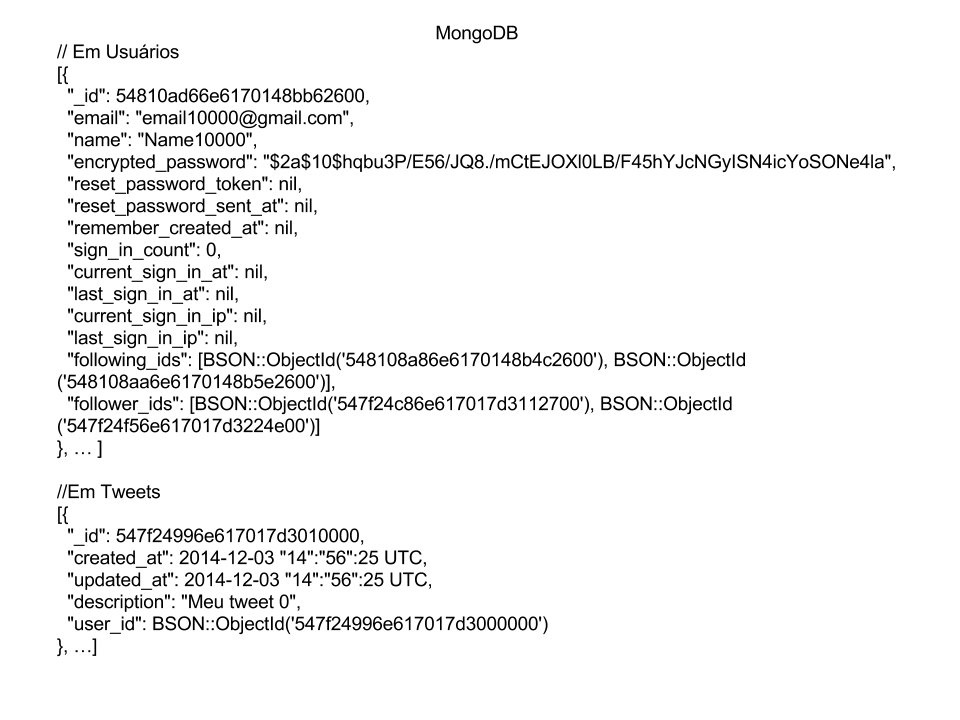
\includegraphics[width=0.8\textwidth]{./04-figuras/data_mono.png}
    \label{fig:data_mono}
\end{figure}


\subsection{Implementação com Persistência Poliglota}
\label{subsec:polyglot}

Para fazer a aplicação com persistência poliglota foi feita uma cópia da aplicação com persistência monoglota e em seguida feitas as alterações necessárias para que o segundo banco de dados fosse usado. O código da aplicação está disponível no GitHub\footnote{\url{https://github.com/zicolimongi/Twitter-Mongo-Redis}}.
Na aplicação monoglota, a única maneira de consultar os \textit{tweets} no \verb|feed| é buscar todos os \textit{tweets}, cujos autores estejam na lista de \verb|followings| do usuário logado. Para isso, era necessário varrer \textit{tweet} por \textit{tweet} e verificar se o autor está na lista. Pensando nessa abordagem utilizamos a persistência poliglota para melhorar o tempo de leitura do \verb|feed| de \textit{tweets}.
Então utilizamos um segundo banco de dados, do gênero chave-valor, chamado \ac{Redis}, que armazena os cem \textit{tweets} mais recentes, cujos autores estão na lista de \verb|followings| do usuário logado.
O \ac{Redis} irá armazenar esses cem \textit{tweets} em uma chave com o identificador do usuário concatenada com a string \verb|"_feed"| , ou seja, se o usuário tiver o identificador igual a um, a chave será \verb|"1_feed"| . Todo usuário terá uma chave que armazenará os \textit{tweets} do \verb|feed|. Quando um for acessar a página de \verb|feed|, ao invés do sistema fazer a consulta no MongoDB e varrer \textit{tweet} por \textit{tweet}, ele irá apenas consultar o \ac{Redis} com a chave e retornará o valor com os cem \textit{tweets} mais recentes que o usuário logado segue.


Para persistir esses dados no \ac{Redis}, precisamos alterar o sistema na camada de controle e na camada de dados. Inicialmente foi necessário instalar outra \textit{gem}, chamada \ac{Redis}\footnote{\url{https://github.com/antirez/redis}}, que faz a comunicação com o banco de dados chave-valor. Em seguida, implementamos três métodos na classe \verb|User|: \verb|feed_key|, \verb|remake_feed| e \verb|update_tweet_hash|, descritos a seguir. O método \verb|feed_key| foi criado apenas para retornar a chave que será usada para armazenar no \ac{Redis}. O método \verb|remake_feed| foi criado para refazer o valor do \verb|feed| de algum usuário quando necessário. Após fazer a implementação poliglota, utilizamos esse método para popular o \ac{Redis}. O método \verb|update_tweet_hash| foi implementado para adicionar mais um \textit{tweet} no \verb|feed| de \textit{tweets} do usuário.

Também precisamos adicionar três métodos na classe \verb|Tweet|: o método \verb|feed_of|, \verb|to_redis_json|,\verb|update_hash|. O método \verb|feed_of| é estático, pois irá trazer uma coleção de \textit{tweets}. Esse método recebe como parâmetro um usuário, acessa o \ac{Redis} com a chave desse usuário e em seguida, faz um parse do valor lido, que foi armazenado como JSON, para aplicação. O método \verb|to_redis_json| é usado para converter o objeto \textit{tweet} no formato JSON para que possa ser armazenado no \ac{Redis}. Por fim, o terceiro método criado é o \verb|update_hash|, privado, que é responsável por atualizar todas as chaves com o \textit{tweet} que foi criado. Esse método é executado por uma função \textit{callback}, chamada \verb|after_create|, com isso, toda a vez que for criado um \textit{tweet} pela aplicação o método \verb|update_hash| será executado.

Ainda foi necessário modificar o controle de \textit{tweet}, para que a ação \verb|feed| leia os \textit{tweets} do \ac{Redis} e não do MongoDB. Todos os dados continuam sendo persistidos no MongoDB, logo eles estão dispostos da mesma maneira do sistema monogolota, \autoref{fig:data_mono}. Já no redis, os dados ficarão dispostos como na \autoref{fig:data_poli}. Apenas os \textit{tweets} são armazenados no \ac{Redis}.
\begin{figure}[H]
    \centering
    \caption{Disposição de dados no sistema com persistência poliglota}
    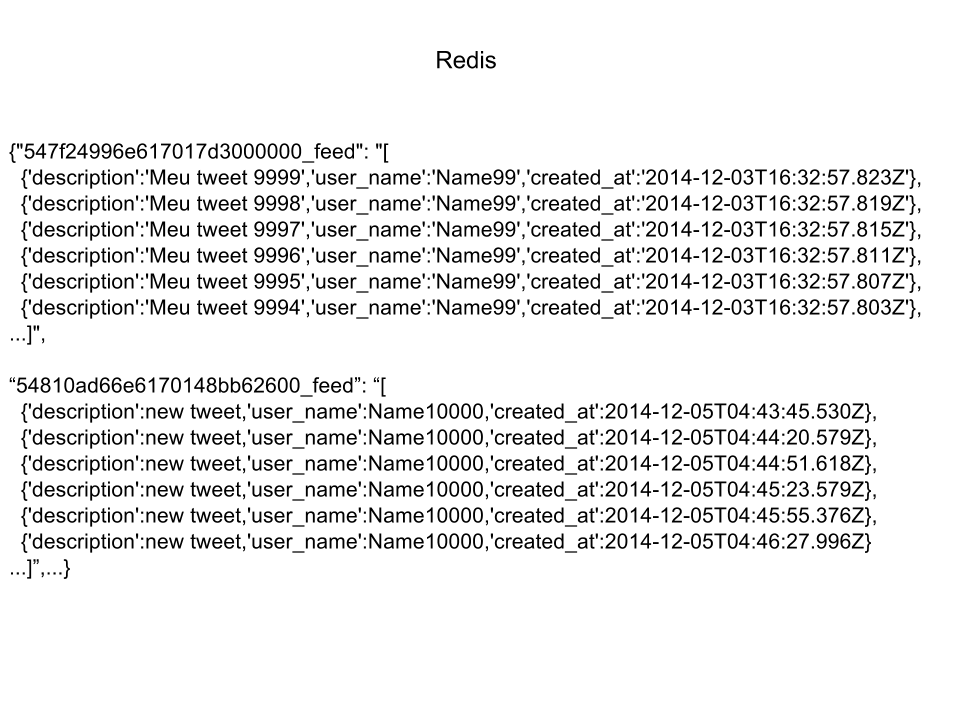
\includegraphics[width=0.8\textwidth]{./04-figuras/data_poli.png}
    \label{fig:data_poli}
\end{figure}





